% !TEX TS-program = pdflatex
% !TEX encoding = UTF-8 Unicode

% This is a simple template for a LaTeX document using the "article" class.
% See "book", "report", "letter" for other types of document.

\documentclass[10pt]{article} % use larger type; default would be 10pt

\usepackage[utf8]{inputenc} % set input encoding (not needed with XeLaTeX)

%%% Examples of Article customizations
% These packages are optional, depending whether you want the features they provide.
% See the LaTeX Companion or other references for full information.

%%% PAGE DIMENSIONS
\usepackage{geometry} % to change the page dimensions
\geometry{letterpaper} % or letterpaper (US) or a5paper or....
\geometry{margin=1.5in} % for example, change the margins to 2 inches all round
% \geometry{landscape} % set up the page for landscape
%   read geometry.pdf for detailed page layout information

\usepackage{graphicx} % support the \includegraphics command and options
\usepackage{mathrsfs}
% \usepackage[parfill]{parskip} % Activate to begin paragraphs with an empty line rather than an indent

%%% PACKAGES
\usepackage{booktabs} % for much better looking tables
\usepackage{array} % for better arrays (eg matrices) in maths
\usepackage{paralist} % very flexible & customisable lists (eg. enumerate/itemize, etc.)
\usepackage{verbatim} % adds environment for commenting out blocks of text & for better verbatim
\usepackage{subfig} % make it possible to include more than one captioned figure/table in a single float
\usepackage[font=small,labelfont=bf]{caption} % Required for specifying captions to tables and figures
% These packages are all incorporated in the memoir class to one degree or another...

%%% HEADERS & FOOTERS
\usepackage{fancyhdr} % This should be set AFTER setting up the page geometry
\pagestyle{fancy} % options: empty , plain , fancy
\renewcommand{\headrulewidth}{0pt} % customise the layout...
\lhead{}\chead{}\rhead{}
\lfoot{}\cfoot{\thepage}\rfoot{}

%%% SECTION TITLE APPEARANCE
\usepackage{sectsty}
\allsectionsfont{\sffamily\mdseries\upshape} % (See the fntguide.pdf for font help)
% (This matches ConTeXt defaults)

%%% ToC (table of contents) APPEARANCE
\usepackage[nottoc,notlof,notlot]{tocbibind} % Put the bibliography in the ToC
\usepackage[titles,subfigure]{tocloft} % Alter the style of the Table of Contents
\renewcommand{\cftsecfont}{\rmfamily\mdseries\upshape}
\renewcommand{\cftsecpagefont}{\rmfamily\mdseries\upshape} % No bold!
\newcommand{\centerfig}[2]{\begin{center}\includegraphics[width=#1\textwidth]{#2}\end{center}}
\usepackage{amssymb}
\usepackage{mathtools}
\DeclarePairedDelimiter\ceil{\lceil}{\rceil}
\DeclarePairedDelimiter\floor{\lfloor}{\rfloor}
\let\oldemptyset\emptyset
\let\emptyset\varnothing
\usepackage[usenames, dvipsnames]{color}
\makeatletter
\def\@maketitle{%
  \newpage
  \null
  \vskip 1em%
  \begin{center}%
  \let \footnote \thanks
	\vskip -5em%
    {\LARGE \@title \par}%
    \vskip 1em
    {\large
      \lineskip .5em%
      \begin{tabular}[t]{c}%
        \@author
      \end{tabular}\par}%
    \vskip 1em%
    {\large \@date}%
  \end{center}%
  \par
  \vskip 1.5em}
\makeatother
%%% END Article customizations

%%% The "real" document content comes below...

\title{Physics 410: Homework 3}
\author{Arnold Choa -- 32038144}
\date{22 October, 2018} % Activate to display a given date or no date (if empty),
         % otherwise the current date is printed 
%{\color{red}{\normalsize{\textbf{TODO}}}} %TODO signage
\begin{document}
\maketitle
\vspace{-0.5cm}
\noindent \Large{Question 1}
\\ \\
\normalsize{Please see \texttt{q1.py} in the \texttt{code} folder for the relevant code.}
\\ \\
\normalsize{The first thing we want to do is to find the 7-point centred formula using a Lagrange interpolant. Given 7 points: $x^* + nh; n=-3,-2,-1,0,1,2,3$} where $x^*$ is our center point, our Lagrange interpolant will be:
\begin{equation}
	p_N(x) = \sum_{n=-3}^{3}F(x^* + nh)L_n(x)
\end{equation}
\begin{equation}
	L_n(x) = \prod_{j \neq n}\frac{(x - x^* - jh)}{(n-j)h}
\end{equation}
Differentiating $p_N(x)$ with respect to x, we get the formula:
\begin{equation}
	p_N'(x) = \sum_{n=-3}^{3}F(x^* + nh)L'_n(x)
\end{equation}
\begin{equation}
	L'_n(x) = \sum_{k \neq  n}\frac{1}{(n-k)h}\prod_{j \neq \{n,k\}}\frac{(x - x^* - jh)}{(n-j)h}
\end{equation}
Solving specifically for the derivative at $x^*$, we get':
\begin{equation}
	p_N'(x^*) = \sum_{n=-3}^{3}F(x^* + nh)L'_n(x^*)
\end{equation}
\begin{equation}
	L'_n(x^*) = \sum_{k \neq  n}\frac{1}{(n-k)h}\prod_{j \neq \{n,k\}}\frac{(- jh)}{(n-j)h} = \frac{1}{h} \sum_{k \neq  n}\frac{1}{n-k}\prod_{j \neq \{n,k\}}\frac{- j}{n-j}
\end{equation}
We can simplify $L'_n(x^*)$ by noting that $\prod_{j \neq \{n,k\}}\frac{- j}{n-j} = 0$ if $k,n \neq 0$. Thus:
\begin{equation}
	L'_n(x^*) =
	\begin{cases}
		\frac{1}{nh} \prod_{j \neq \{n,0\}}\frac{- j}{n-j}; n \neq 0 \\
		\frac{1}{h} \sum_{k \neq  0} -\frac{1}{k}\prod_{j \neq \{0,k\}}\frac{- j}{0-j} =\frac{1}{h} \sum_{k \neq  0} -\frac{1}{k} ; n=0
	\end{cases}
Solving for our weights:
\end{equation}
\[
\begin{array}{c | c }
L'_{-3}(x^*)	&	-\frac{1}{3h} \cdot \frac{(2)(1)(-1)(-2)(-3)}{(-1)(-2)(-4)(-5)(-6)} = 	-\frac{1}{h} \cdot \frac{12}{240} = -\frac{1}{h} \cdot \frac{1}{60}\\
L'_{-2}(x^*)	&	-\frac{1}{2h} \cdot \frac{(3)(1)(-1)(-2)(-3)}{(1)(-1)(-3)(-4)(-5)}	= 	\frac{1}{h} \cdot \frac{18}{60} = \frac{1}{h} \cdot \frac{3}{20}\\
L'_{-1}(x^*)	&	-\frac{1}{1h} \cdot \frac{(3)(2)(-1)(-2)(-3)}{(2)(1)(-2)(-3)(-4)} = -\frac{1}{h} \cdot \frac{36}{48} = -\frac{1}{h} \cdot \frac{3}{4}\\
L'_{0}(x^*)	&	\frac{1}{h} \left( \left(\frac{1}{3} + \frac{1}{2} + \frac{1}{1}\right) - \left(\frac{1}{3} + \frac{1}{2} + \frac{1}{1}\right)\right) = 0\\
L'_{1}(x^*)	&	\frac{1}{1h} \cdot \frac{(3)(2)(1)(-2)(-3)}{(4)(3)(2)(-1)(-2)}	= \frac{1}{h} \cdot \frac{36}{48} = \frac{1}{h} \cdot \frac{3}{4}\\
L'_{2}(x^*)	&	\frac{1}{2h} \cdot \frac{(3)(2)(1)(-1)(-3)}{(5)(4)(3)(1)(-1)}	= 	-\frac{1}{h} \cdot \frac{18}{60} = -\frac{1}{h} \cdot \frac{3}{20}\\
L'_{3}(x^*)	&	\frac{1}{3h} \cdot \frac{(3)(2)(1)(-1)(-2)}{(6)(5)(4)(2)(1)} = \frac{1}{h} \cdot \frac{12}{240} = \frac{1}{h} \cdot \frac{1}{60}		
\end{array}
\]
Thus, for the 7-point centred formula:
\begin{equation}
	p_N'(x^*) = \frac{1}{h} \left[
	\begin{aligned}
	&\frac{1}{60}(F(x^* + 3h) - F(x^* - 3h)) - \frac{3}{20}(F(x^* + 2h) - F(x^* - 2h)) + \\
	&\frac{3}{4}(F(x^* + h) - F(x^* - h))
	\end{aligned}
	\right]
\end{equation}

\noindent Now, trying to estimate the error for the 7-point centred formula, we note that for a 7-point Richardson formula of the same form and coefficients, we have an error of:
\begin{equation}
	\epsilon = Ch^7 + \frac{M}{h}
\end{equation}
where $M$ is the Machine Precision and $C$ is an unknown constant 1 (we usually assume $C=1$ to get a ballpark figure). Minimizing the function we find that:
\begin{equation}
	\epsilon' = C7h^6 - \frac{M}{h^2} = 0
\end{equation}
which is $0$ when:
\begin{equation}
	h = \sqrt[8]{\frac{M}{C7}}
\end{equation}
Seeing that Python's machine precision for floats is in the order of magnitude of $M \approx 2 * 10^{-16}$, our error will be minimized when we choose an $h \approx 8 * 10^{-3}$ within an error of an order of magnitude. After solving for a ballpark figure of our optimal $h$, we can start plotting and estimating our errors.
\\ \\
Estimating the derivative of $f(x) = \sin(x^2)$, we know that analytically, $f'(x) = 2x\cos(x^2)$. Plotting our approximation, the actual derivative, and the accumulated error:
\begin{center}
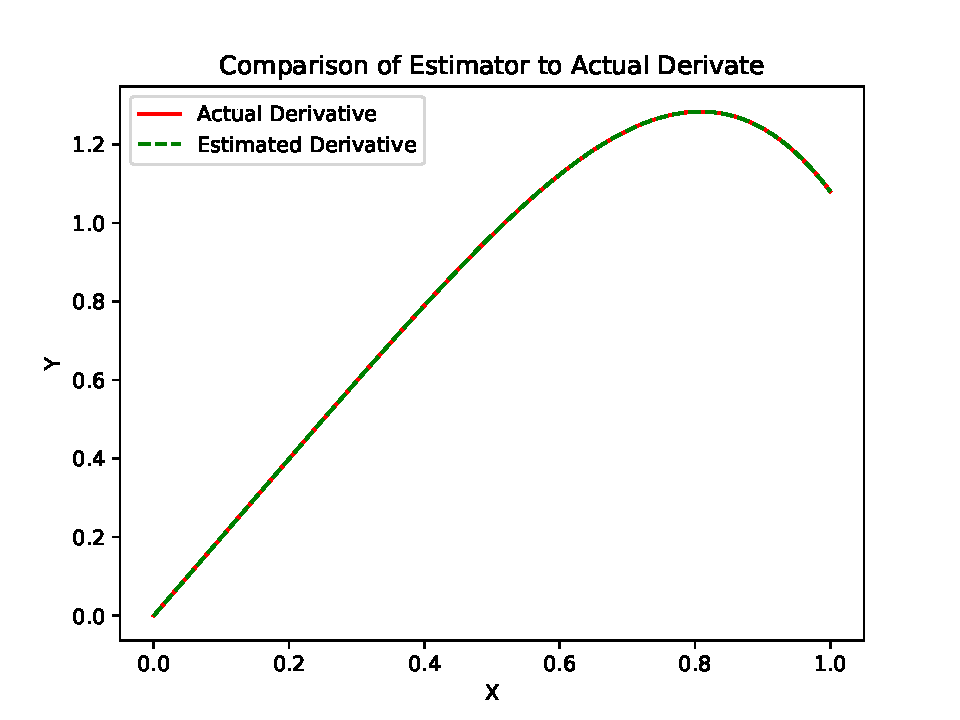
\includegraphics[width=.45\textwidth]{../figs/q1_comparison.pdf}
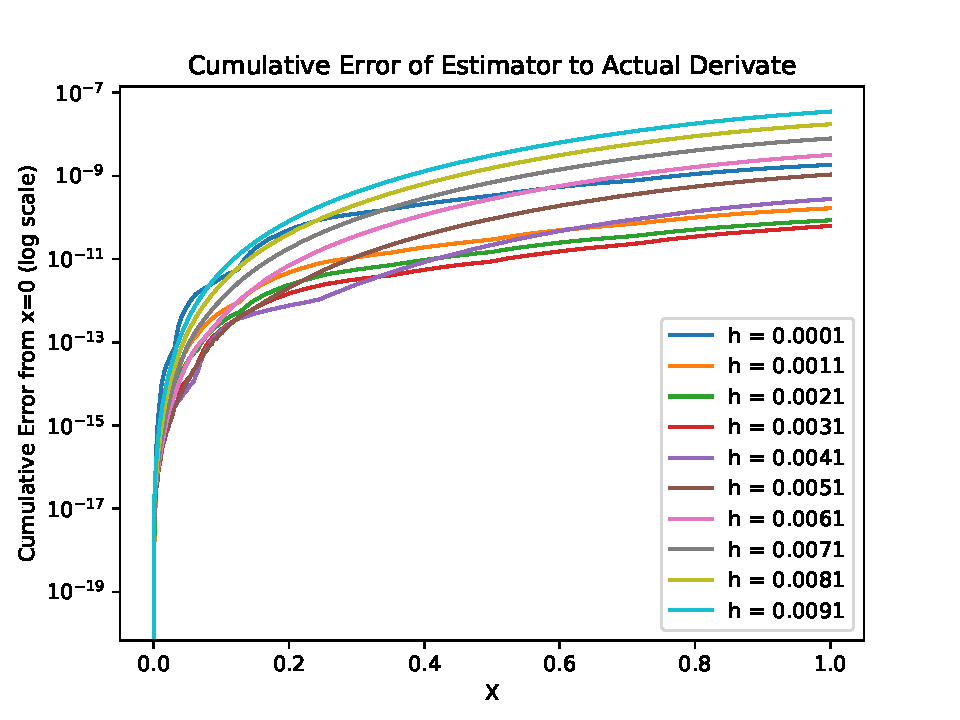
\includegraphics[width=.45\textwidth]{../figs/q1_error.pdf}
\end{center}
\captionof{figure}{Comparison and Error Plots of the Estimated Derivative versus the Actual Derivative. At the  comparison plot, I used $h=0.003$ as suggested by the cumulative error plot.}
\vspace{1em}
 It can be noted that 0.003 was within an order of magnitude of our ballpark estimation of the minimizer at $h^* = 0.008$ which is within expectation due to the constant $C$. We see that using $h=0.003$, our accumulated error is $\approx  6 * 10^{-11}$ taken with $10^{4}$ datapoints, leaving us an average error of $6 * 10^{-15}$ which is an order of magnitude from our our machine precision of $\approx 2 * 10^{-16}$.
\newpage
\noindent \Large{Question 2}
\\ \\
\normalsize{Please see \texttt{q2.py} in the \texttt{code} folder for the relevant code.}
\\ \\
The composite trapezoid formula dictates that given an integral $f(x)$, a range $[a,b]$, and $N$ being the number of sub-intervals:
\begin{equation}
	\int_{a}^{b}f(x)dx \approx \frac{b-a}{N}\left( \frac{f(x_0)}{2} + f(x_1) + f(x_2) + \ldots + f(x_{N-1})+\frac{f(x_N)}{2} \right)
\end{equation}
In generality, the Romberg integration approximation with parameters $m,k$ can be written as:
\begin{equation}
	\int_{a}^{b}f(x)dx \approx T_{m,k} = \frac{4^k T_{m,k-1} - T_{m-1,k-1}}{4^k - 1}
\end{equation}
where $T_{m,0}$ denotes the composite trapezoid formula with $N = 2^{m}$ sub-intervals. The trapezoid rule removes all odd orders of error, and so this formula, given $k$, will remove errors up until the order of $h^{2(k+1)}$. To get rid of all error up to $h^6$, we would need $k\geq2.$
\\ \\
Going through multiple iterations of $m$, the closest approximation I could get, just by eliminating all errors up to the order of $h^6$, was at $m=19; k=2$. This gave me the approximate integral value of $0.4596976941318603$ which had an error of $5.551115123125783E-17$ from the original integral.
\end{document}
